\documentclass[conference]{IEEEtran}



\usepackage{graphicx}
\usepackage{subfigure}
\usepackage{graphicx}
\usepackage{caption}



\hyphenation{op-tical net-works semi-conduc-tor}


\begin{document}

\title{Distributed Online Training Simulation for Railway Dispatcher }



\author{\IEEEauthorblockN{Nuri Ozalp, Ahmet Basgoze, Ozdemir Kavak, Burcu Kalkan}
\IEEEauthorblockA{TUBITAK BILGEM\\Informatics and Information Security\\ Research Center\\
Kocaeli, Turkey 41470\\
Email: {(nuri.ozalp, ahmet.basgoze, ozdemir.kavak, burcu.kalkan)}@tubitak.gov.tr}


}

\maketitle

\begin{abstract}
Computer Simulations can be considered as a powerful tools for learning such as analysing, designing, and interacting. Especially in the vital criticality level it has become more important tools such as train traffic simulation.
The most important purpose of the train control system to prevent train collisions with other trains, keeping them in safe range.

The purpose of this study is to provide train traffic control in a distributed simulation system. The system consists of an instructor five students and a scenario-editor. The system use real train route model located in Turkey.  During the simulation, dispatchers console can controls train traffic which have different  size and speed in system. Success in educational outcomes can be measured. Instructor console make decisions about the organization of teaching and learning 
experiences, classroom management, and responses to 
individual students. The user is able to monitor and track the progress of five targeted students throughout the course of the simulation.

nuriiii nuriiii nuriiii

burcu burcu burcu
\end{abstract}

\section{INTRODUCTION}
Kara ve Demiryolu taşımacılığında önemli bir yeri bulunan tren, bir ya da birkaç lokomotif tarafından çekilen, itilen ve vagonlardan oluşan bir ulaşım aracıdır. Ulaşım ve taşımacılık anlanlarında trenlerin çok önemli bir yere sahip olduğu bilinen bir gerçektir. 
Artan demiryolu trafiği sonucunda Dünya genelinde değişik trafik kontrol sistemleri geliştirilmiştir. Tren trafiği yönetim metotlarının dünyada birçok farklı merkezi tren trafik kontrol sistemleri vardır.


Demiryolu trafiği yönetimi için kullanılan sistemler merkezi kontrol sistemleri olup, kontrolörler (dispeçer) tarafında idare edilmektedir.  Dispeçerlerin amaçları trenleri güvenle ve zamanında varması gereken hedeflere ulaştırmaktır.


Tren trafiği kontrol sistemleri çok kritik sistemlerdir.Anlık konum bilgisi eski model trenlerde bilinmemektedir. Sinyalizasyon sistemleri sayesinde trenlerin yaklaşık konumları 3km civarında tahmin edilebilmektedir. Bu nedenle tren trafiği kritik olmaktadır. Son yıllarda dispeçer eğitimi sefer sayılarının artması ve tren yollarının artması ile daha da önem kazanmıştır. Dispeçerlerin gerçek tren trfiği üzerinde çalışarak tecrübe kazanmaları hemuzun zaman almakta hem de birtakım riskleri beraberinde getirmektedir. Bu nedenle eğitim simülasyon sistemlerine ihtiyaç duyulmaktadır ve birçok eğitim simulasyonu geliştirilmiştir. Özellikle kontrol merkezlerinde birden çok dipeçerin birlikte çalışmasından dolayı dağıtık yapılı ve birden çok kullanıcılı simulasyonlar önem kazanmıştır. Bu sayede tek bir simulasyonda hazırlanan yoğun trafikli senaryo ile birden çok dispeçerin birlikte tren trafiği yönetmesi ve birçok problemle başa çıkması önem arz etmektedir. 


Bu çalışmada dispeçerlerin geliştirilen simülasyon sistemi altyapısı kullanılarak eğitilmesi ve gerçek tren trafiği yönetimine hazır hale getirilmesi ve daha kısa sürede alanında uzmanlaşabilmesi hedeflenmiştir. Simülasyon ortamında yoğun trafikli, farklı tip ve hızlardaki trenlerin bulunduğu demiryolu sahası oluşturularak bu saha üzerinde meydana gelebilecek problemler oluşturulmakta ve yapılan tüm bu işlemler senaryo olarak kaydedilmektedir. Kaydedilen senoryolar eğitmen tarafından açılarak aynı anda 5 öğrenciye kadar eğitim verilmesine ve sonrasında öğrencilerin performanslarının  değerlendirilerek karne verilmesine imkan sağlamaktadır.


Geliştirilen simülasyon siteminde  Türkiye'deki 3 farklı tipteki gerçek tren hattı çizimleri yapılmışve  sisteme tanıtılmıştır. Bunlarda 1 tanesi hızlı Tren hattı, bir diğeri banliyo hattı ve sonuncusu geleneksel tren hattı ndan olşmaktadır. 3 farklı tipteki tren hattına ait karakterisitik farklılıklar kullanılarak öğrencilerin eğitilmesi halihazırdaki sistem tarafından gerçekleştirilmektedir.


Geliştirilen simülasyon sistemi 5 modülden oluşmaktadır. 
Bunlar; 
\begin{itemize}
\item eğitmen konsolu,
\item öğrenci konsolu, 
\item seneryo editörü,
\item performans değerlendirme modülü,
\item tren graf modülüdür. 
\end{itemize}




Seneryo editörü ile istenilen arazi hazırlanmakta ve istenilen kadar farklı konumlara tren eklenebilmekte ve istenilen bütün koşullar bu arazide oluşturulmaktadır.Arazide oluşturulabilecek koşullar çarpışma, bölge zaman izni, deray, kırmızı sinyal ihlali, kırmızı geçiş, lokomotif arızası, tren/vagon kaçması, sinyal arızası, makas arızası, sürat tecavüzü, hemzemin geçit arızası gibi durumları içermektedir. Oluşturulan senaryo ile eğitmen ister tek simülasyon isterse farklı 5 simülasyon olarak aynı anda başlatabilmekte ve simülasyonlara müdahele edebilmektedir. İstediği zaman snapshot ile eğitimde bazı önemli gördüğü yerleri tekrar tekrar öğrencilere tecrübe ettirebilmektedir. Öğrenciler yetkileri ölçüsünde sorumlu olduğu alanda tren trafiğini yönetebilmekte ve meydana gelen arızaların çözümü için çalışmalar yapabilmektedir. Simülasyondaki trenlerin anlık hareketleri aynı zamanda trengraf ile takip edebilmektedir. Eğitim sonunda eğitmen öğrencilerin performansını ölçmek amaçlı değerlendirme yapılabilmekte ve yetiştirilen dispeçerin başarısı puanlama sistemi ve başarılı/başarısız olarak ölçülebilmektedir.


2. bölümde related work ler ile ilgili , 3. bölümde sistemin haberleşme alt yapısı hakkında bilgiler verilmiştir. 4. Bölümde sisteme ait 5 modülden bahsedilmiştir. 5. modülde sistem üzerinde yapılan deney ve sonuçları hakkında bilgiler yer almaktadır. 6.bölümde ise sonuç kısmına yer verilmiştir.




\section{RELATED WORK}


Tren trafiğini yöneten ve birden çok dispeçerin eğitim aldığı dağıtık yapılı simülasyonlar yaygın olarak kullanılmaktadır.Benzer çalışmalara bu bölümde yer verilmiştir.


In Middelkoop and his friend study is a simulator which which stands for Flexible Rail Infra Simulation of Operations (FRISO). It includes automatized  a simulation model by using a connection to database, editor including generator functions and the possibility to perform single and multiple (stochastic) simulation experiments. FRISO models include following elements  track layout, signalling system, route setting, and interlocking. Our system presents multiple screen of regions and to let five students to work at same or different simulation at the same time \cite{FRISO}.

 


In Baohua  and his friend's study is about  multi-train simulator. It is able to do  train performances assessment at the given railway lines, signal layouts optimization, energy-efficient operating strategies , in major terminals exploration of traffic bottlenecks, the evaluation of the reliability of scheduled timetables and train delay propagation. In multi-train simulation does these automatically, in our system dispatcher conduct them \cite{ICVES}.




\section{SYSTEM DESIGN}
\subsection{Simülasyon Yaşam Döngüsü}

RAYTES sistemi beş bağımsız simülasyon ortamını eşzamanlı ve birbirinden bağımsız olarak yürütebilmektedir. Aşağıdaki gösterilen Şekil \ref{fig:simyasamdongusu}' deki yaşam döngüsü bir simülasyon ortamını temsil etmektedir. Sistem ilk çalıştırıldğında IDLE durumda bulunmaktadır. Bir senaryo sisteme yüklenerek simülasyon oturumu oluşturulduğunda LOADED durumuna geçilir. Bu durumda simülasyon başlangıç saatinde beklemekte olup, çalışmaya hazır haldedir. Simülasyon çalıştırıldığında RUNNING durumuna geçer. RUNNING durumunda simülasyon saati ilerlemekte, simüle edilen nesneler zamana duyarlı biçimde akmakta ve insan arayüzlerinde sistem ile kullanıcılar arası etkileşim gerçeklenmektedir. Simülasyon herhangi bir zamanında duraksatılabilir, bu durumda simülasyon PAUSE durumuna geçer. PAUSE durumunda iken simülasyon saati ve simülasyon işlemleri geçici olarak durdurulur. PAUSE durumunda yine simülasyon RUNNING durumuna başlayabilir. Simülasyon sonlandırıldığında TERMINATED durumuna düşer ve simülasyon artık yeniden başlatılamaz.




\begin{figure}[h!]
  \centering
  % Requires \usepackage{graphicx}
  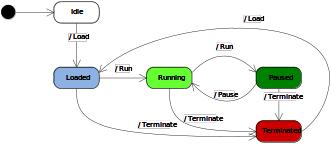
\includegraphics[width=8cm]{simyasamdongusu.jpg}
  \caption{Representation of Simulation Life cycle}\label{fig:simyasamdongusu}
\end{figure}

\subsection{Comminication}
\subsubsection{ Simulation Message}
Simulation Message mesaj türü simülasyon sistemin üst seviye kumanda ve kontrol merkezi mesajlaşma türüdür. Bu mesajlar Eğitmen Konsolu’nda üretilmektedir ve sistemin diğer bileşenlerine gönderilmektedir. Simülasyon’un yaratılması, duraklatılması, snapshot alınması, gibi temel simülasyon komutlarını içermektedir. Ayrıca simülasyondaki sanal saha nesnelerinin durumlarına müdahale etmek amacıyla bir takım özel müdahale komutları tanımlıdır. Mesaj komutları Tablo 1 de verilmektedir.
\subsubsection{Request Message}
RequestMessage mesaj türü Kontrol Merkezi Client (KMC) modülünün Kontrol Merkezi Sunucu (KMS) modülüne gönderilen komutları taşımaktadır. KMC ve KMS arasındaki protokol “client-server” mimarisi olup RequestMessage komutları istemci tarafın sunucu tarafından hizmet isteği olarak değerlendirilmektedir. RequestMessage komutları Tablo x te listelenmektedir.

\subsubsection{State Message}

StateMessage mesajlar simülasyon çalışması esnasında sanal saha daki tanımlı elemanların durum bilgilerinin iletilmesi için kullanılmaktadır. Kontrol Merkezi Sunucu (KMS) modülü StateMessage kullanlarak Kontrol Merkezi Client (KMC) modülüne saha bilgilerini göndermektedir. Kontrol Merkezi Sunucu ayriyetten saha görüntüleme ihtiyacı duyan Geniş Ekran Konsolu (GEK) ve Eğitmen Saha Müdahale (ESM) modüllerine de StateMessage vasıtasıyla bilgi göndermektedir.

\subsubsection{System Message}
SystemMessage mesajlar Öğrenci Kontrol Yönetimi (ÖKY) ile Kontrol Merkezi Sunucu (KMS) modüller arası kullanılan mesajlaşmadır. Bu mesaj türü öğrenci olarak eğitim sistemine dahil olmak isteyen kullanıcıların giriş (login) yapmasını sağlamakta kullanılmaktadır.

\subsection{Modbus}
Modbus otomasyon sanayi çevrelerinde kabul görmüş bir ham veri iletişim protokoludür. Bu protokol “client-server” mantığında çalışıp sistemler arası bit dizilerin sorgulanması ve iletilmesinde kullanılmaktadır. RAYTES projesinde Modbus paketler UDP/IP üzerinden yazılım modülünden diğer modüllere iletilmektedir. Kontrol Merkezi Sunucu (KMS) modülü, Anklaşman Simülatör (AS) modülü, Saha Simülatör (SS) modülü ve Tren Simülatör (TS) modüller arası komut ve bilgi transferi Modbus paketler ile gerçekleşmektedir.


\subsection{SSY Simülasyon Sunucu Yönetim Modülü}
SSY yani Simülasyon Sunucu Yönetim modülü simülasyon sistemi içerisindeki tüm aktif modüllerin bağlı olduğu haberleşme altyapısının bulunduğu ve koordinasyonun sağlandığı modüldür.Şekil \ref{fig:syySequenceDiagram}'de squance diagram ve  Şekil \ref{fig:syygrafic}'de arayüzü gösterilmiştir.
Simülasyon akışı içerisinde doğrudan bir görevle sorumlu tüm aktif modüller bu modüle ya doğrudan ya da altında çalıştıkları ana modül üzerinden dolaylı olarak bağlı olmak zorundadır. Simülasyonun çalışması ve hazırlanması esnasında gerçekleşen tüm mesajlaşmalar bu modül üzerinden gerçekleşmektedir.
SSY ayrıca sistemdeki aktif konsollar gibi kendi içerisindeki bilgileri uygun mesajlara karşılık olarak diğer konsollarla yada uygulamalarla paylaşabilmektedir.
SSY mesajlaşma amacıyla tüm sistem elemanları gibi SD yani Simülasyon Destek ve Mesajlaşama Modülü’nü kullanmaktadır. Bu birim tüm giriş bilgilerini SD üzerinden almakta olup yine çıkış bilgilerini de SD üzerinden sisteme dağıtmaktadır. SD bu SSY üzerinde Mesaj Sunucu görevi ile tanımlanmış olarak kullanılmaktadır.
SSY üzerine gelen herbir mesaj bir ön kontrolden geçirilerek mesaj ile ilgili yapılması gereken işleme karar verilir. SSY’nin bir mesaj üzerine yapacağı 4 işlem vardır;

\begin{itemize}
\item Mesajı doğrudan hedef ya da hedeflerine göndermek
\item Mesajı tüm ağa yayınlamak
\item Mesajın içeriği SSY ile ilgili ise SSY’den doğrudan cevap mesajı yollamak
\item Mesajın hiyerarşik olarak göderilmesi gerekiyorsa bu hiyerarşinin sağlanması
\end{itemize}






\begin{figure}[h!]
  \centering
  % Requires \usepackage{graphicx}
  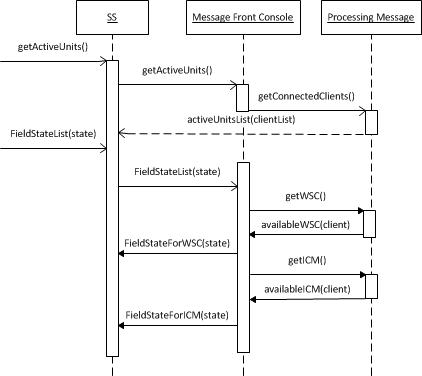
\includegraphics[width=8cm]{syySequenceDiagram.jpg}
  \caption{Representation of SYY squence diagram}\label{fig:syySequenceDiagram}
\end{figure}


\begin{figure}[h!]
  \centering
  % Requires \usepackage{graphicx}
  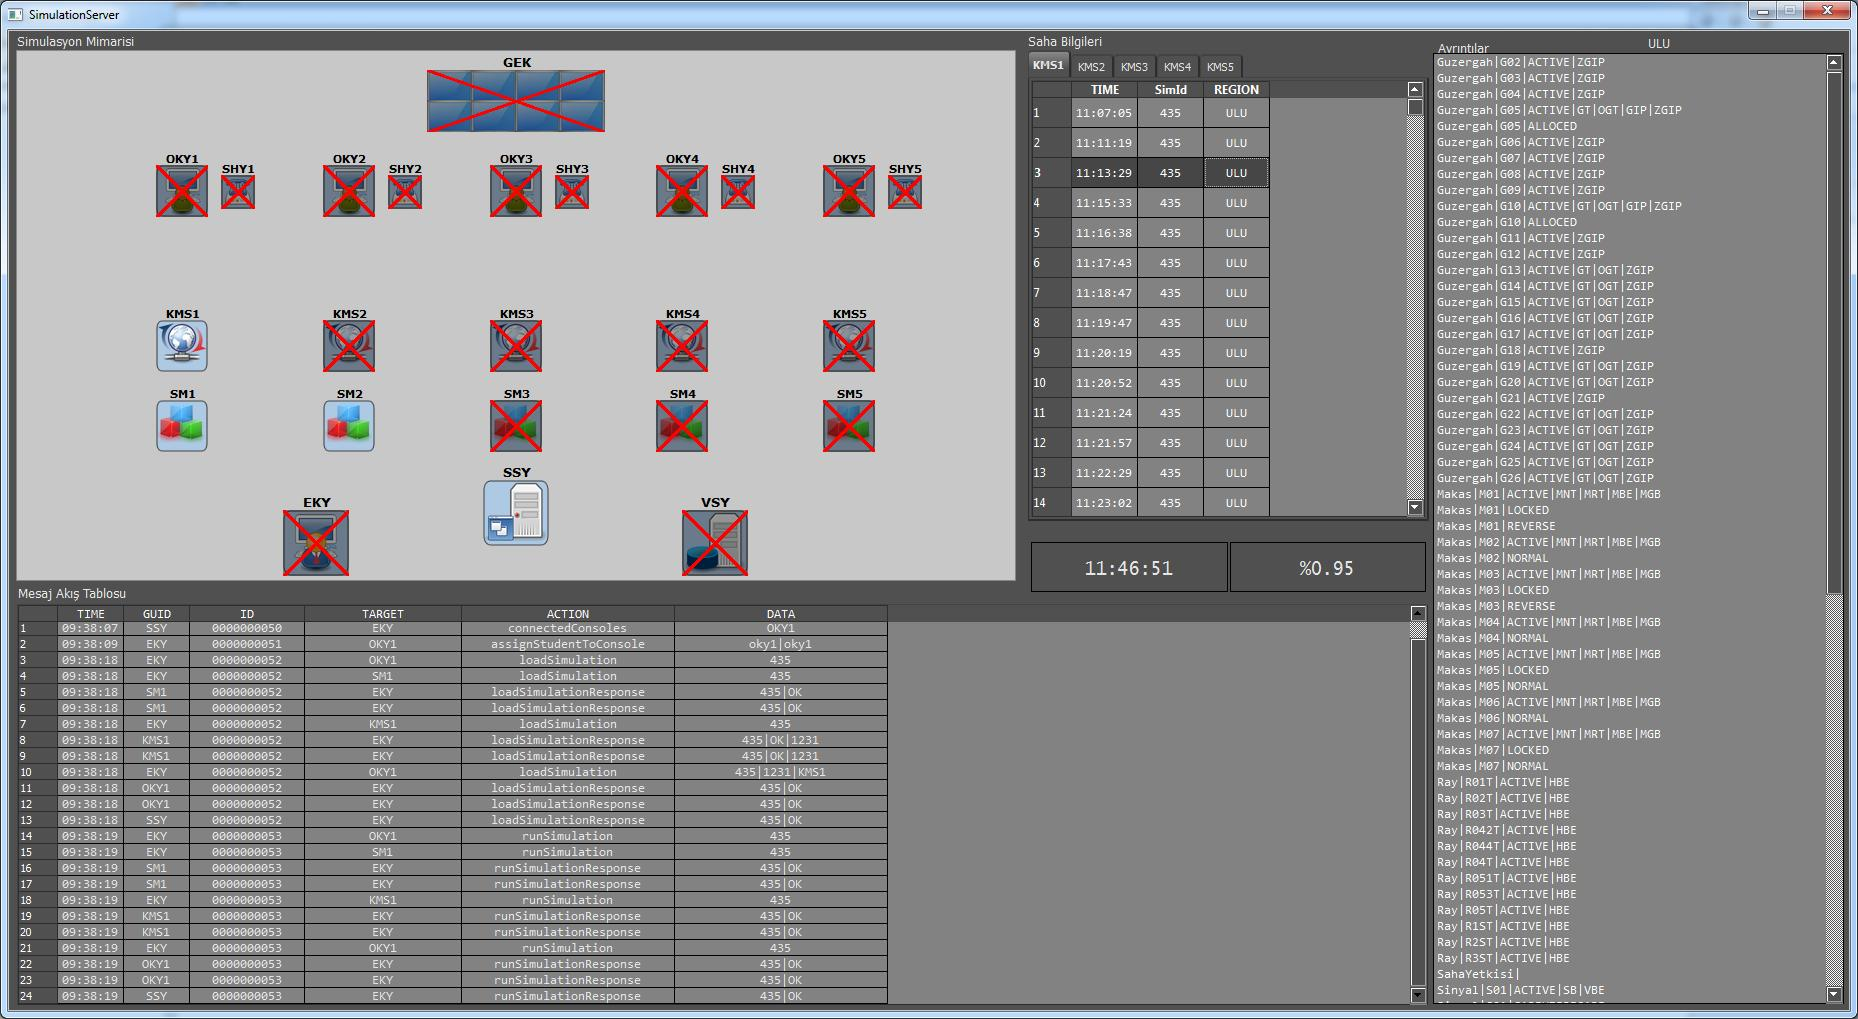
\includegraphics[width=8cm]{syygrafic.jpg}
  \caption{Representation of SYY UI}\label{fig:syygrafic}
\end{figure}




Hiyerarşik mesaj gönderimi bir mesajın, örneğin simülasyon yükleme mesajının öncelik sırasına göre her bir birime yollanması anlamına gelmektedir. Sıra ile yollanan her bir mesaj sonrasında olumlu cevap gelmesi durumunda bir sonraki ilgili birime mesaj iletilir. Bu zincir bir noktada kırılırsa sistem mesajı gönderen ilk birime olumsuz mesajı döndürür. Eğer mesaj zinciri tamamlanırsa olumlu mesajı iletilir.

\subsection{SM Simülasyon Motor Modülü}
\subsubsection{Sınıf Yapısı}
Simülasyon Motoru (SM) modülündeki Şekil \ref{fig:smgrafic}'de gösterilen ana sınıf SimMotor sınıfıdır. Bu sınıf Config, XmlUtility, SahaEventList, FTSimManager::FTSimMgr ve Communicator::Client sınıfları bünyesinde yaratıp kullanmaktadır. FTSimMgr Saha Trafik Simülasyon Yönetimi (FTS) modülünde tanımlıdır. SimMotor sınıfı FTSimMgr sınıfın sağladığı arayüz üzerinden anklaşman, saha ve trafik simülasyon modellerine erişmektedir. Communicator modüllünde tanımlı Client sınıfı ise SimMotor sınıfına SimulationMessage mesajlaşma arayüz sağlamaktadır. SimMotorGui, SimMotor sınıfa debug ve test maksatlı grafik pencere arayüzü sağlamaktadır.

\begin{figure}[h!]
  \centering
  % Requires \usepackage{graphicx}
  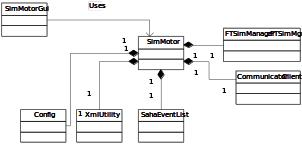
\includegraphics[width=8cm]{smgrafic.jpg}
  \caption{Representation of SM class diagram}\label{fig:smgrafic}
\end{figure}



\subsubsection{Mesajlaşma}
Simülasyon Sunucu Yönetimi (SSY) ilk başladığında 5 adet bağımsız Simülasyon Motoru (SM) proses yaratır. Bu SM proses’ler sayesinde 5 bağımsız simülasyon eşzamanlı olarak SSY tarafından kontrol edilmesine olanak sağlar. SSY SimulasyonMessage tür mesajarı SM ye aktarmaktadır. Bu tür mesajlar, simülasyon yükle, sümülasyon başlat tarzında üst seviye kontrol mesajlarıdır. SM bu mesajları Saha Trafik Yönetimi (FTS) simülasyon modüllerine iletmektedir. Simülasyon modülü bu mesajların gerektirdiği işlemleri tamamladığında SM’ye yanıt (olumlu veya olumsuz) vermektedir ve bu netice SSY ye geri bildirilmektedir.
LoadSimulation mesajı genel örnek olarak ele alınırsa; bu mesaj SM tarafından alındığında iki işlem tetiklemektedir. Birincisi, senaryo da oynatılması gereken önceden programlanmış olaylar veritabanından okunuyor ve Saha Event List (SEL) listesine yüklenmektedir. Bu olayların her biri bir Saha Event (SE) olarak tanımlanmıştır. 
İkinci işlem ise FTS ve onun bünyesindeki Saha Simülasyon (SS) modeli, Anklaşman Simülasyon (AS) modeli ve Trafik Simülasyon (TS) modelini ilgili senaryonun teknik parametrelerini veritabanından yüklemesi ve simülasyon başlatma durumu için hazırlanması.
Simülasyon Running durumundayken SEL deki sıralanmış SE olaylar simülasyon zamanına göre FTS modülüne işlenmek için aktarılmaktadır. Bu mekanizma bir senaryonun müdahalesiz olarak işlenmesini sağlamaktadır. Ancak bir simülasyona ayrıca eğitmen tarafından müdahale edilmesine olanak vermektedir. Eğitimen, Eğitmen Saha Müdahale (ESM) aracı kullanarak manuel Saha Event yaratabilir. Bu manuel olarak yaratılan SE olaylar SM’ye anlık olarak iletdiğinde SE olayı SEL listesinin başına eklemektedir ve böylelikle simülasyon’un sonraki çevriminde hemen işlenmesi sağlanmaktadır. Bütün bu akış Şekil \ref{fig:smCommunicationDiagram}'deki diagramda gösterilmiştir.

\begin{figure}[h!]
  \centering
  % Requires \usepackage{graphicx}
  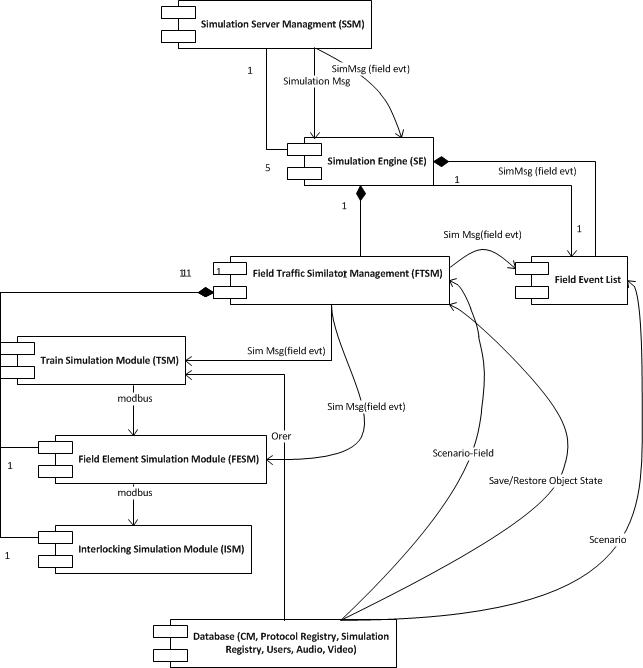
\includegraphics[width=8cm]{smCommunicationDiagram.jpg}
  \caption{Representation of SM Comminication diagram}\label{fig:smCommunicationDiagram}
\end{figure}

\subsubsection{SD Simülasyon Destek ve Mesajlaşma Modülü}

Şekil \ref{fig:RepresentationSDDiagram}'de görüldüğü gibi Simülasyon Destek ve Mesajlaşma modülü proje içerisinde birbirinden fiziksel olarak bağımsızlar fakat haberleşme ve etkileşim içinde olan birimlerin birbirleri ile olan haberleşmesini birlikte sağlamaktadır.
Temel sunucu istemci mimarisi üzerine kurulmuş haberleşme modülü projeye özgü bağlantı kopukluğu kontrolü, tekil bağlantı özelliği, XML tabanlı mesaj kontrolü gibi özellikler eklenerek projeye özgü protokol kuralları çerçevesinde tasarlanmıştır.
Mesajlaşma ve iletişimi sağlayacak olan ana modül iki modda çalışabilmektedir. Bu modalardan ilki Server yani sunucu mod iken diğer mod ise Client yani istemci modüldür. Sunucu modda çalıştırıldığında belirli bir bağlantı portu üzerinden haberleşmenin sağlandığı bu sistem diğer yani İstemci modda diğer sistemlerin bağlanmasını beklenmektedir.  

\begin{figure}[h!]
  \centering
  % Requires \usepackage{graphicx}
  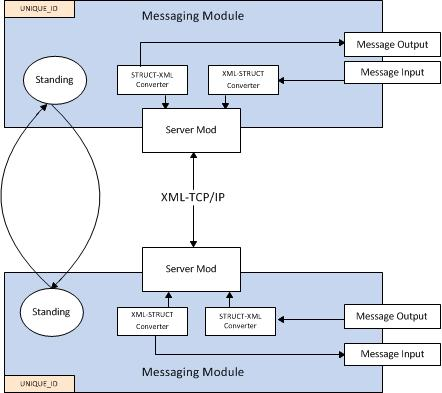
\includegraphics[width=8cm]{RepresentationSDDiagram.jpg}
  \caption{Representation of SD  diagram}\label{fig:RepresentationSDDiagram}
\end{figure}

İstemci mod bağlantı esnasında hedef sunucu bilgilerini ve kendisini tanıtan tekil eşsiz bir ID ile erişimi sağlayacaktır. Bu bağlantıları eşsiz hale getirmek için IP numaraları kullanılmayacaktır. Çünkü aynı makina üzerindeki farklı uygulamalar birbirleri ile sunucu üzerinden haberleşme yeteneğine sahip olmalıdır. Aynı ID ile birden fazla erişim denemesi yapıldığında sistem 2. sistemin bağlantı denemesini “Kullanımdaki bir ID” uyarsıyla reddedecektir. 
Şekil \ref{fig:SDDiagram}'de görüldüğü gibi yine bir sunucuya bağlı olan tüm istemciler o sunucuya periyodik olarak sunucuya bağlı oldukları yani ayakta oldukları bilgisini yollarlar. Ters açıdan bakıldığında sunucu da kendisine bağlı olan tüm istemcilere çalışır yani ayakta olduğu bilgisini periyodik olarak bildirmektedir. Bu sayede sistemdeki tüm elemanların bağlantı kontrolü gerçekleştirebilecektir. 


\begin{figure}[h!]
  \centering
  % Requires \usepackage{graphicx}
  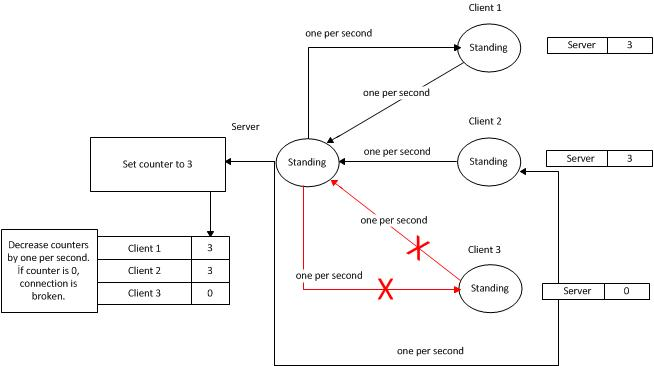
\includegraphics[width=8cm]{SDDiagram.jpg}
  \caption{Representation of SD  diagram}\label{fig:SDDiagram}
\end{figure}




\section{Training Environment}

\subsection{ÖK Öğrenci Konsolu}

Öğrenci Konsolu (ÖK) bir Öğrenci Bilgisayarı (ÖBÜ) ve bir Sesli Haberleşme Cihazı (SHC) alt donanım bileşenlerden oluşmaktadır. ÖK’nin yapısı Şekil \ref{fig:ogrenci}'de gösterilmiştir.
Öğrenci Konsol Yönetimi (ÖKY) yazılım modülü üst seviye modül olup konsolunun genel işlevlerinden sorumludur. Dispeçer arayüz uygulamasını KM Client (KMC) modülü gerçekleştirmektedir. Ekranların video görüntü kayıtları Video Kayıt Altyapı (VKA) modülü tarafından gerçekleştirilmektedir.
Sesli Haberleşme Cihazı dispeçerin sesli iletişimini sağlamak için gerekli mikrofon, kulaklık veya telefon ahizesi ile donatılacak ve üzerinde çalışan Sesli Haberleşme Yazılım Modülü (SHY) eğitim amaçlarına uygun biçimde arama yapmayı, aranmayı destekleyecektir. 

\begin{figure}[h!]
  \centering
  % Requires \usepackage{graphicx}
  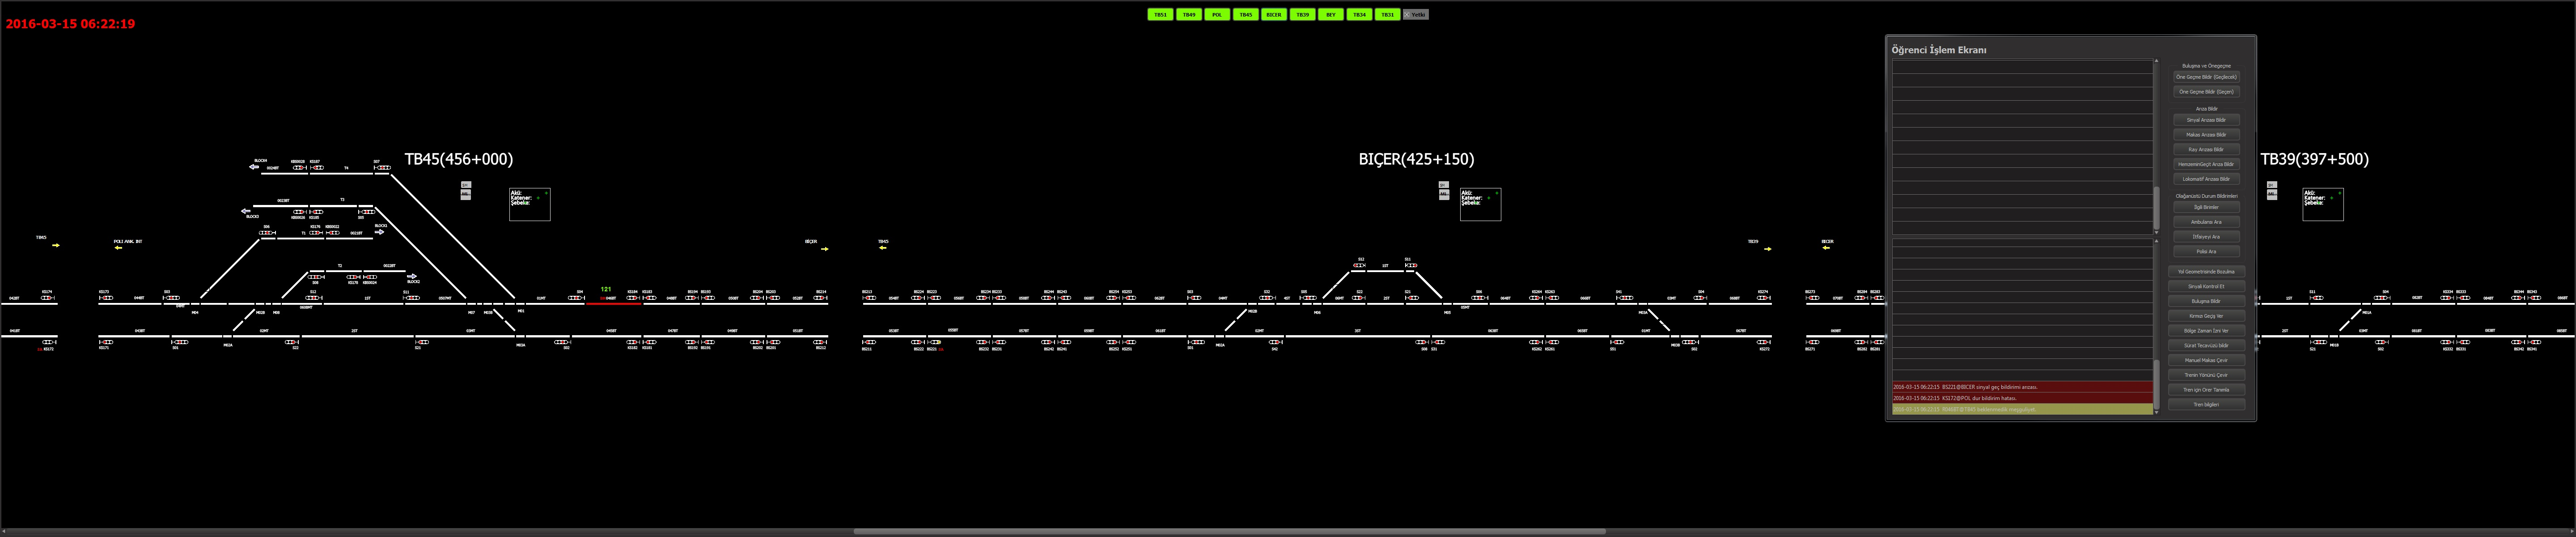
\includegraphics[width=8cm,height=5cm]{ogrenci.jpg}
  \caption{Representation of Dispatcher Console}\label{fig:smclass}
\end{figure}



\subsection{GEK Geniş Ekran Konsolu}

Geniş Ekran Konsolu (GEK) bir Geniş Ekran Bilgisayar Ünitesi (ÖBÜ) ve bir Geniş Ekran Duvar Ünitesi (GDÜ) donanım bileşenlerden oluşmaktadır.GEK’in yapısı Şekil 3 de gösterilmiştir.
Geniş Ekran Bilgisayar Ünitesi (GBÜ) çok çıkışlı ekran kartı ile donatılmış olup, her çıkış Geniş Ekran Duvar ünitesinin birer ekranına bağlıdır. Bilgisayar üzerinde Geniş Ekran Konsol Yönetimi (GKY) yazılımı çalışmaktadır. Bu yazılım Dispeçer arayüz uygulaması olan KM Client (KMC), Video Kayıt Altyapı (VKA) ve Video Geri Oynatma Aracı (VGO) modüllerin çalıştırılması ve kontrol edilmesinden sorumludur.
Geniş Ekran Duvar Ünitesi (GDÜ) iki satır dört sütün düzenine göre yerleştirilmiş 8 LCD ekranlık görüntüleme duvarı şeklinde tasarlanmıştır.
Sesli Haberleşme Cihazı eğitmenin sesli iletişimini sağlamak için gerekli mikrofon, kulaklık veya telefon ahizesi ile donatılacak ve üzerinde çalışan Sesli Haberleşme Yazılım Modülü (SHY) eğitim amaçlarına uygun biçimde arama yapmayı, aranmayı destekleyecektir.
Şekil \ref{fig:genisekranSonuc}'de geniş ekrana ait deney sonucunun ekran görüntüsü görülmektedir.


\subsection{Eğitmen Konsolu}

Eğitmen Konsolu (EK) simülasyon başlatıp simülasyona öğrenci ataması yapabilen ve seneryo atayan roldedir. Simülasyon anında simülasyona müdahele edebilmektedir. Simülasyonu durdurabilir devam ettirilebilir ve sonlandırabilir. Öğrenciden gelen taleplere onay verebilir. Snapshot alabilir. Şekil \ref{fig:egitmenSonuc}'de eğitmen paneli ile yapılan deneye ait ekran görüntüsü yer almaktadır.


\subsection{SSÜ Simülasyon Sunucu Ünitesi}

RAYTES projesinde tüm mesajlaşma koordinasyonu sağlamak amacıyla Simülasyon Sunucu Ünitesi uygulaması kullanılacaktır. Endüstriyel bir sunucu bilgisayarda koşacak uygulama proje ekibi tarafından geliştirilecektir. Uygulamanın temel işlevleri simülasyon bileşenleri arasında mesajlaşma senkronizasyonunu ve koordinasyonu sağlamak, sistemin çalışmasını tüm mesaj akışlarını görüntülemek, simülasyon altyapısını oluşturan diğer sunucu taraflı bileşenlerin ayağa kaldırılmasını sağlamak, simülasyon bileşenlerin bağlantı bilgilerini tutmak ve bunları diğer bileşenlerle paylaşmak gibi görevlerdir. Simülasyon sisteminin tüm aktif bileşenleri Simülasyon sunucusuna doğrudan ya da dolaylı olarak bağlı bulunacaktır.
\subsection{Editör Analiz Konsolu}

Editör Analiz Konsolu üzerinde Senaryo Editör Aracı (SED), Performans Analiz Aracı (PA), Kullanıcı Yönetim Aracı (KYA), Öğrenci Eğitim Kayıtları Aracı (ÖEK) ve Video Geri Oynatma Aracı (VGO) yazılım modüller çalışmaktadır.
EAK simülasyon öncesi senaryoların hazırlanması, kullanıcıların tanımlanması, ve simülasyon sonrası eğitim performans analizi ve öğrenci eğitim kayıtlarını incelemek için kullanılmaktadır. Dolaysıyla bu konsol simülasyon eğitimi esnasında değil “off-line” kullanılmaya yöneliktir.

\subsection{Train Graph}


Raytes Projesi kapsamında geliştirilen Trengraf bileşeni, tren hareket kayıtlarının (TrainEvent) sorgulanarak grafik üzerinde çeşitli seçenekler ile gösterimini sağlayan bir veri analiz aracıdır.
74 de örnek bir ekran görüntüsü verilmiştir. Sorgu sonucunda trenlerin bloklardan geçiş hareketleri rahatlıkla izlenebilmektedir. 


\begin{itemize}
\item Eğrinin solundaki çizgi ile işaretlenmiş noktalar trenin bloklara girişini,
\item Eğrinin sağındaki çizgi ile işaretlenmiş noktalar trenin bloklardan çıkışını,
\item İki çizgi arasında kalan transparan boyalı alan ise giriş-çıkış arasındaki zaman farkını, yani trenin o blokta ne kadar kaldığını ifade etmektedir.
\end{itemize}

Bu seçeneklerin hangilerinin gösterileceği kullanıcı tarafından seçilebilmektedir.
Şekil \ref{fig:trenGrapSonuc}'de tren grafa ait çalıştırılan deney sonucundaki ekran göüntüsü görülmektedir.


\section{EXPERIMENT RESULT}
Geliştirdiğimiz dağıtık yapılı 5 öğrencinin aynı anda eğitim alabildiği RAYTES projemizi 2 şekilde test ettik. Bunlardan ilki 20 tren ve tek simülasyon 5 kullanıcı yetkisi dahilinde 1 saatlik seneryoda eğitim aldılar. Toplam RAM ve CPU kullanımı Şekil \ref{fig:hepsibir}'de gösterilmiştir


\begin{figure}[h!]
  \centering
  % Requires \usepackage{graphicx}
  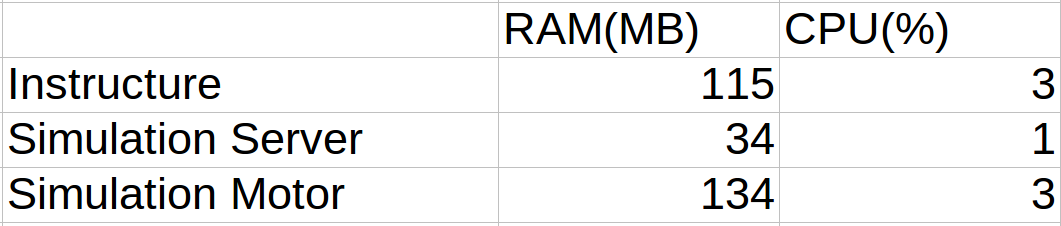
\includegraphics[width=8cm]{hepsibir.png}
  \caption{Tek simülasyon ve 5 farklı öğrenci ile yapılan eğitime ait modüllerin kaynak kullanımını göstermektedir}\label{fig:hepsibir}
  
\end{figure}

Diğer testimizde 1'er saatilik 5 ayrı simülasyon ve her simülasyona bir öğrenci atandı. Bu şekilde eğitim aldılar. Toplam RAM ve CPU kullanımı Şekil \ref{fig:hepsiayri}'de gösterilmiştir

\begin{figure}[h!]
  \centering
  % Requires \usepackage{graphicx}
  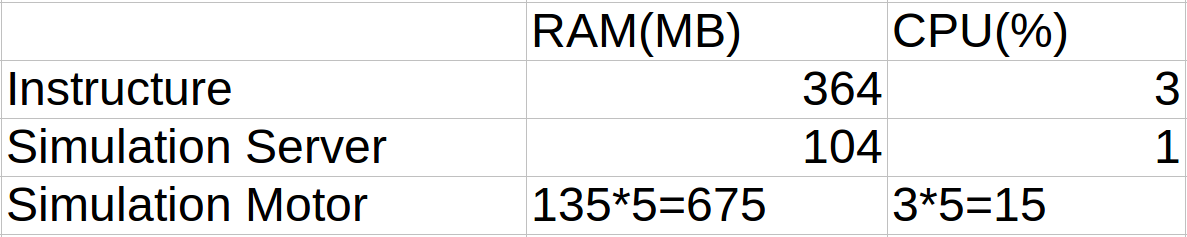
\includegraphics[width=8cm]{hepsiayri.png}
  \caption{5 farklı simülasyon ve 5 farklı öğrenci ile yapılan eğitime ait modüllerin kaynak kullanımını göstermektedir}\label{fig:hepsiayri}
  
\end{figure}

Deneyler sonucunda elde edilen tren hareketlerini gösteren tren graf şekildeki gibi olmaktadır. 
\begin{figure}[h!]
  \centering
  % Requires \usepackage{graphicx}
  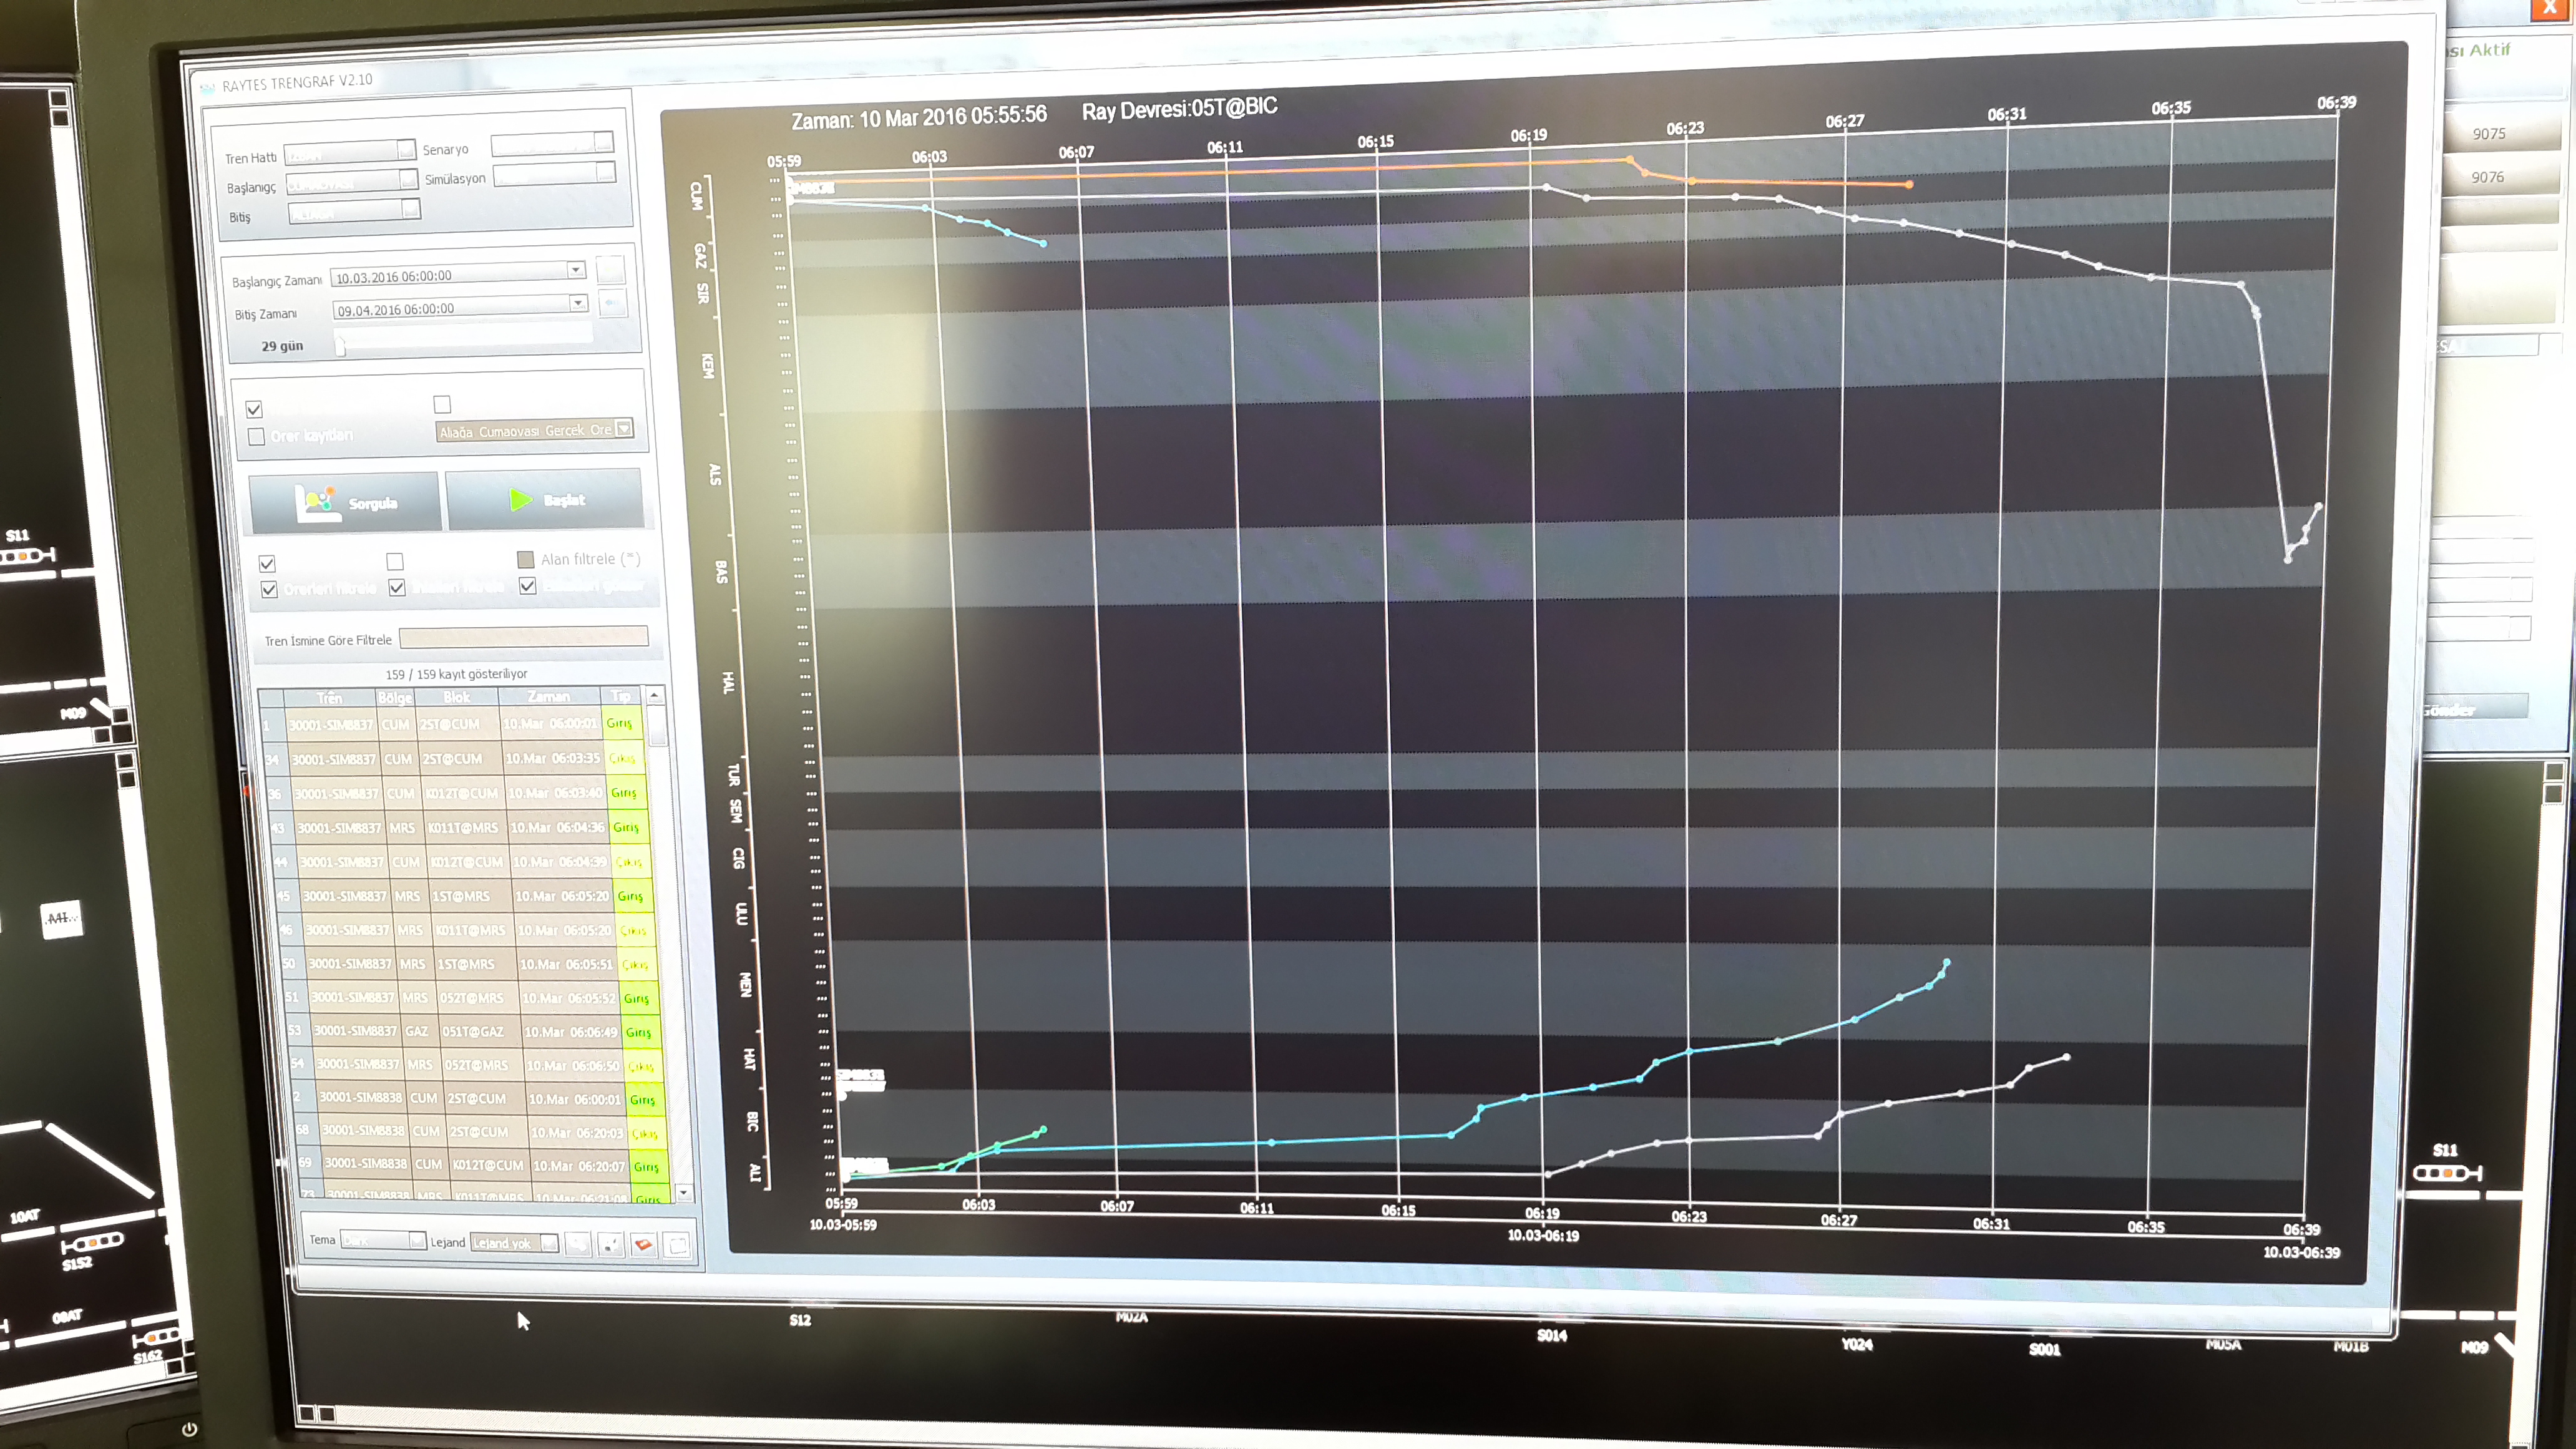
\includegraphics[width=8cm]{trenGrapSonuc.jpg}
  \caption{Tren hareketlerinin gösterimi}\label{fig:trenGrapSonuc}
  
\end{figure}
\begin{figure}[h!]
  \centering
  % Requires \usepackage{graphicx}
  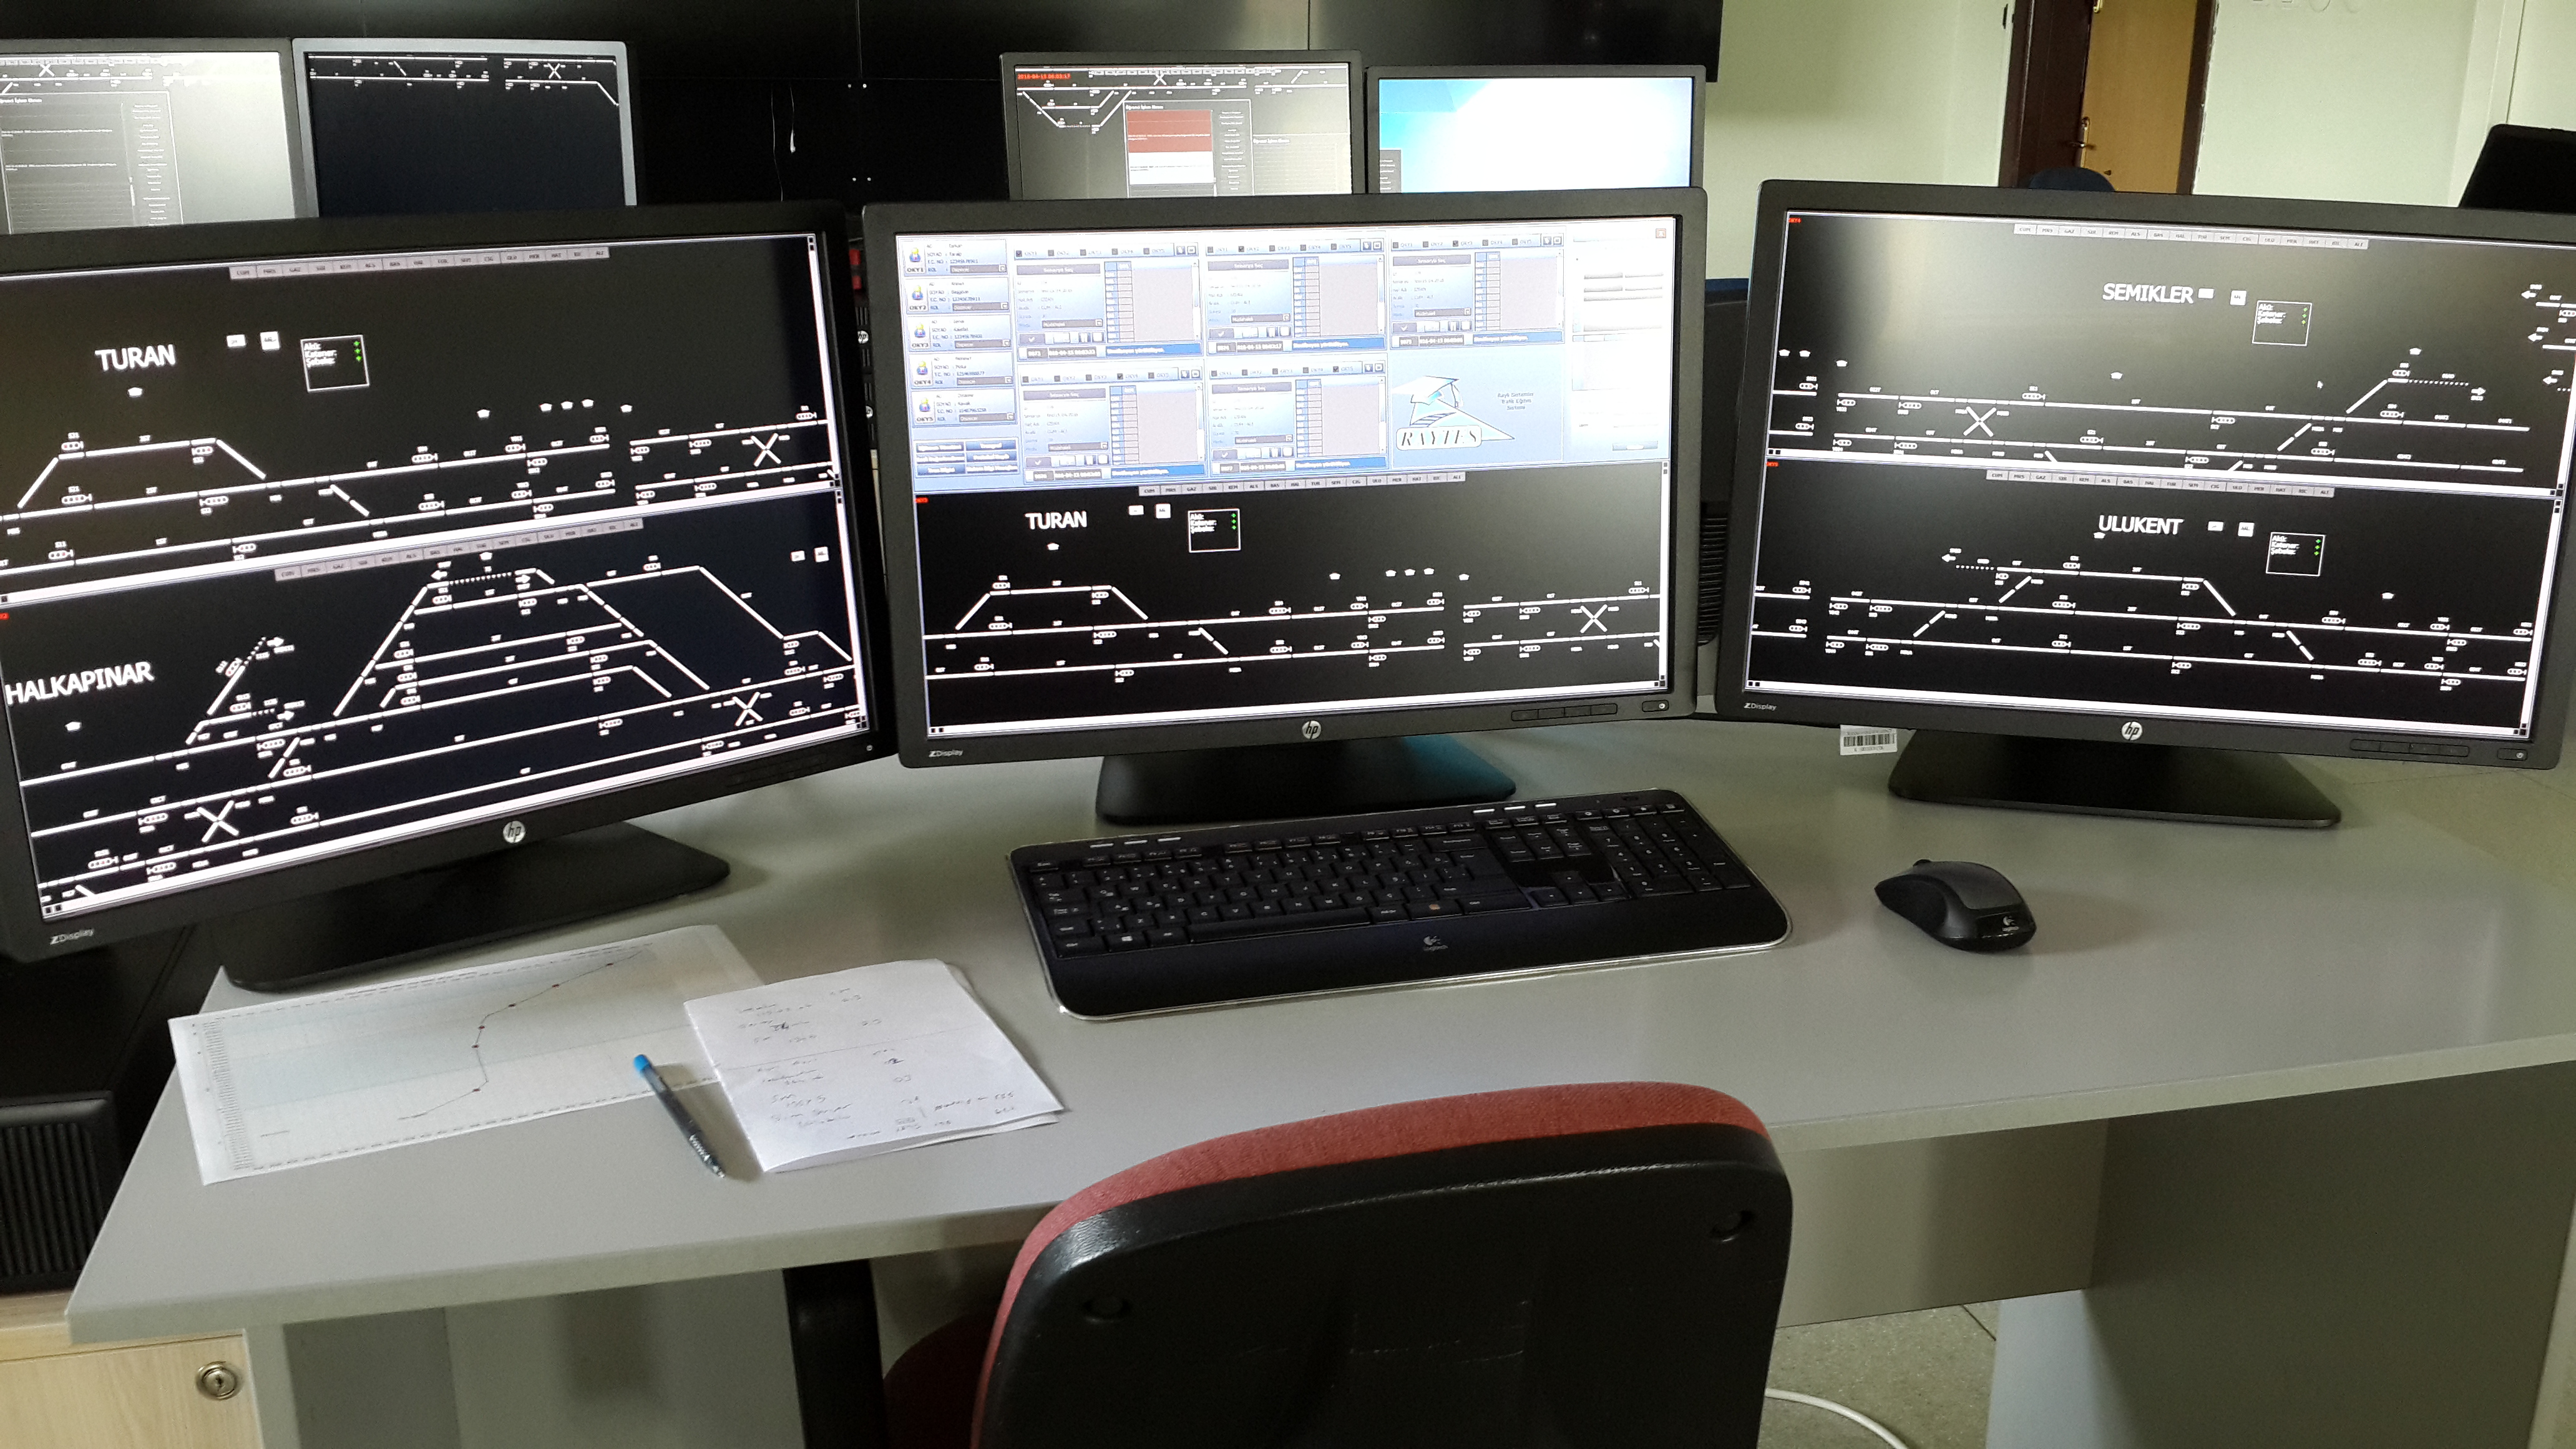
\includegraphics[width=8cm]{egitmenSonuc.jpg}
  \caption{5 farklı simülasyon ve 5 farklı öğrenci ile yapılan eğitimin eğitmen konsolunda gösterimi}\label{fig:egitmenSonuc}
  
\end{figure}
\begin{figure}[h!]
  \centering
  % Requires \usepackage{graphicx}
  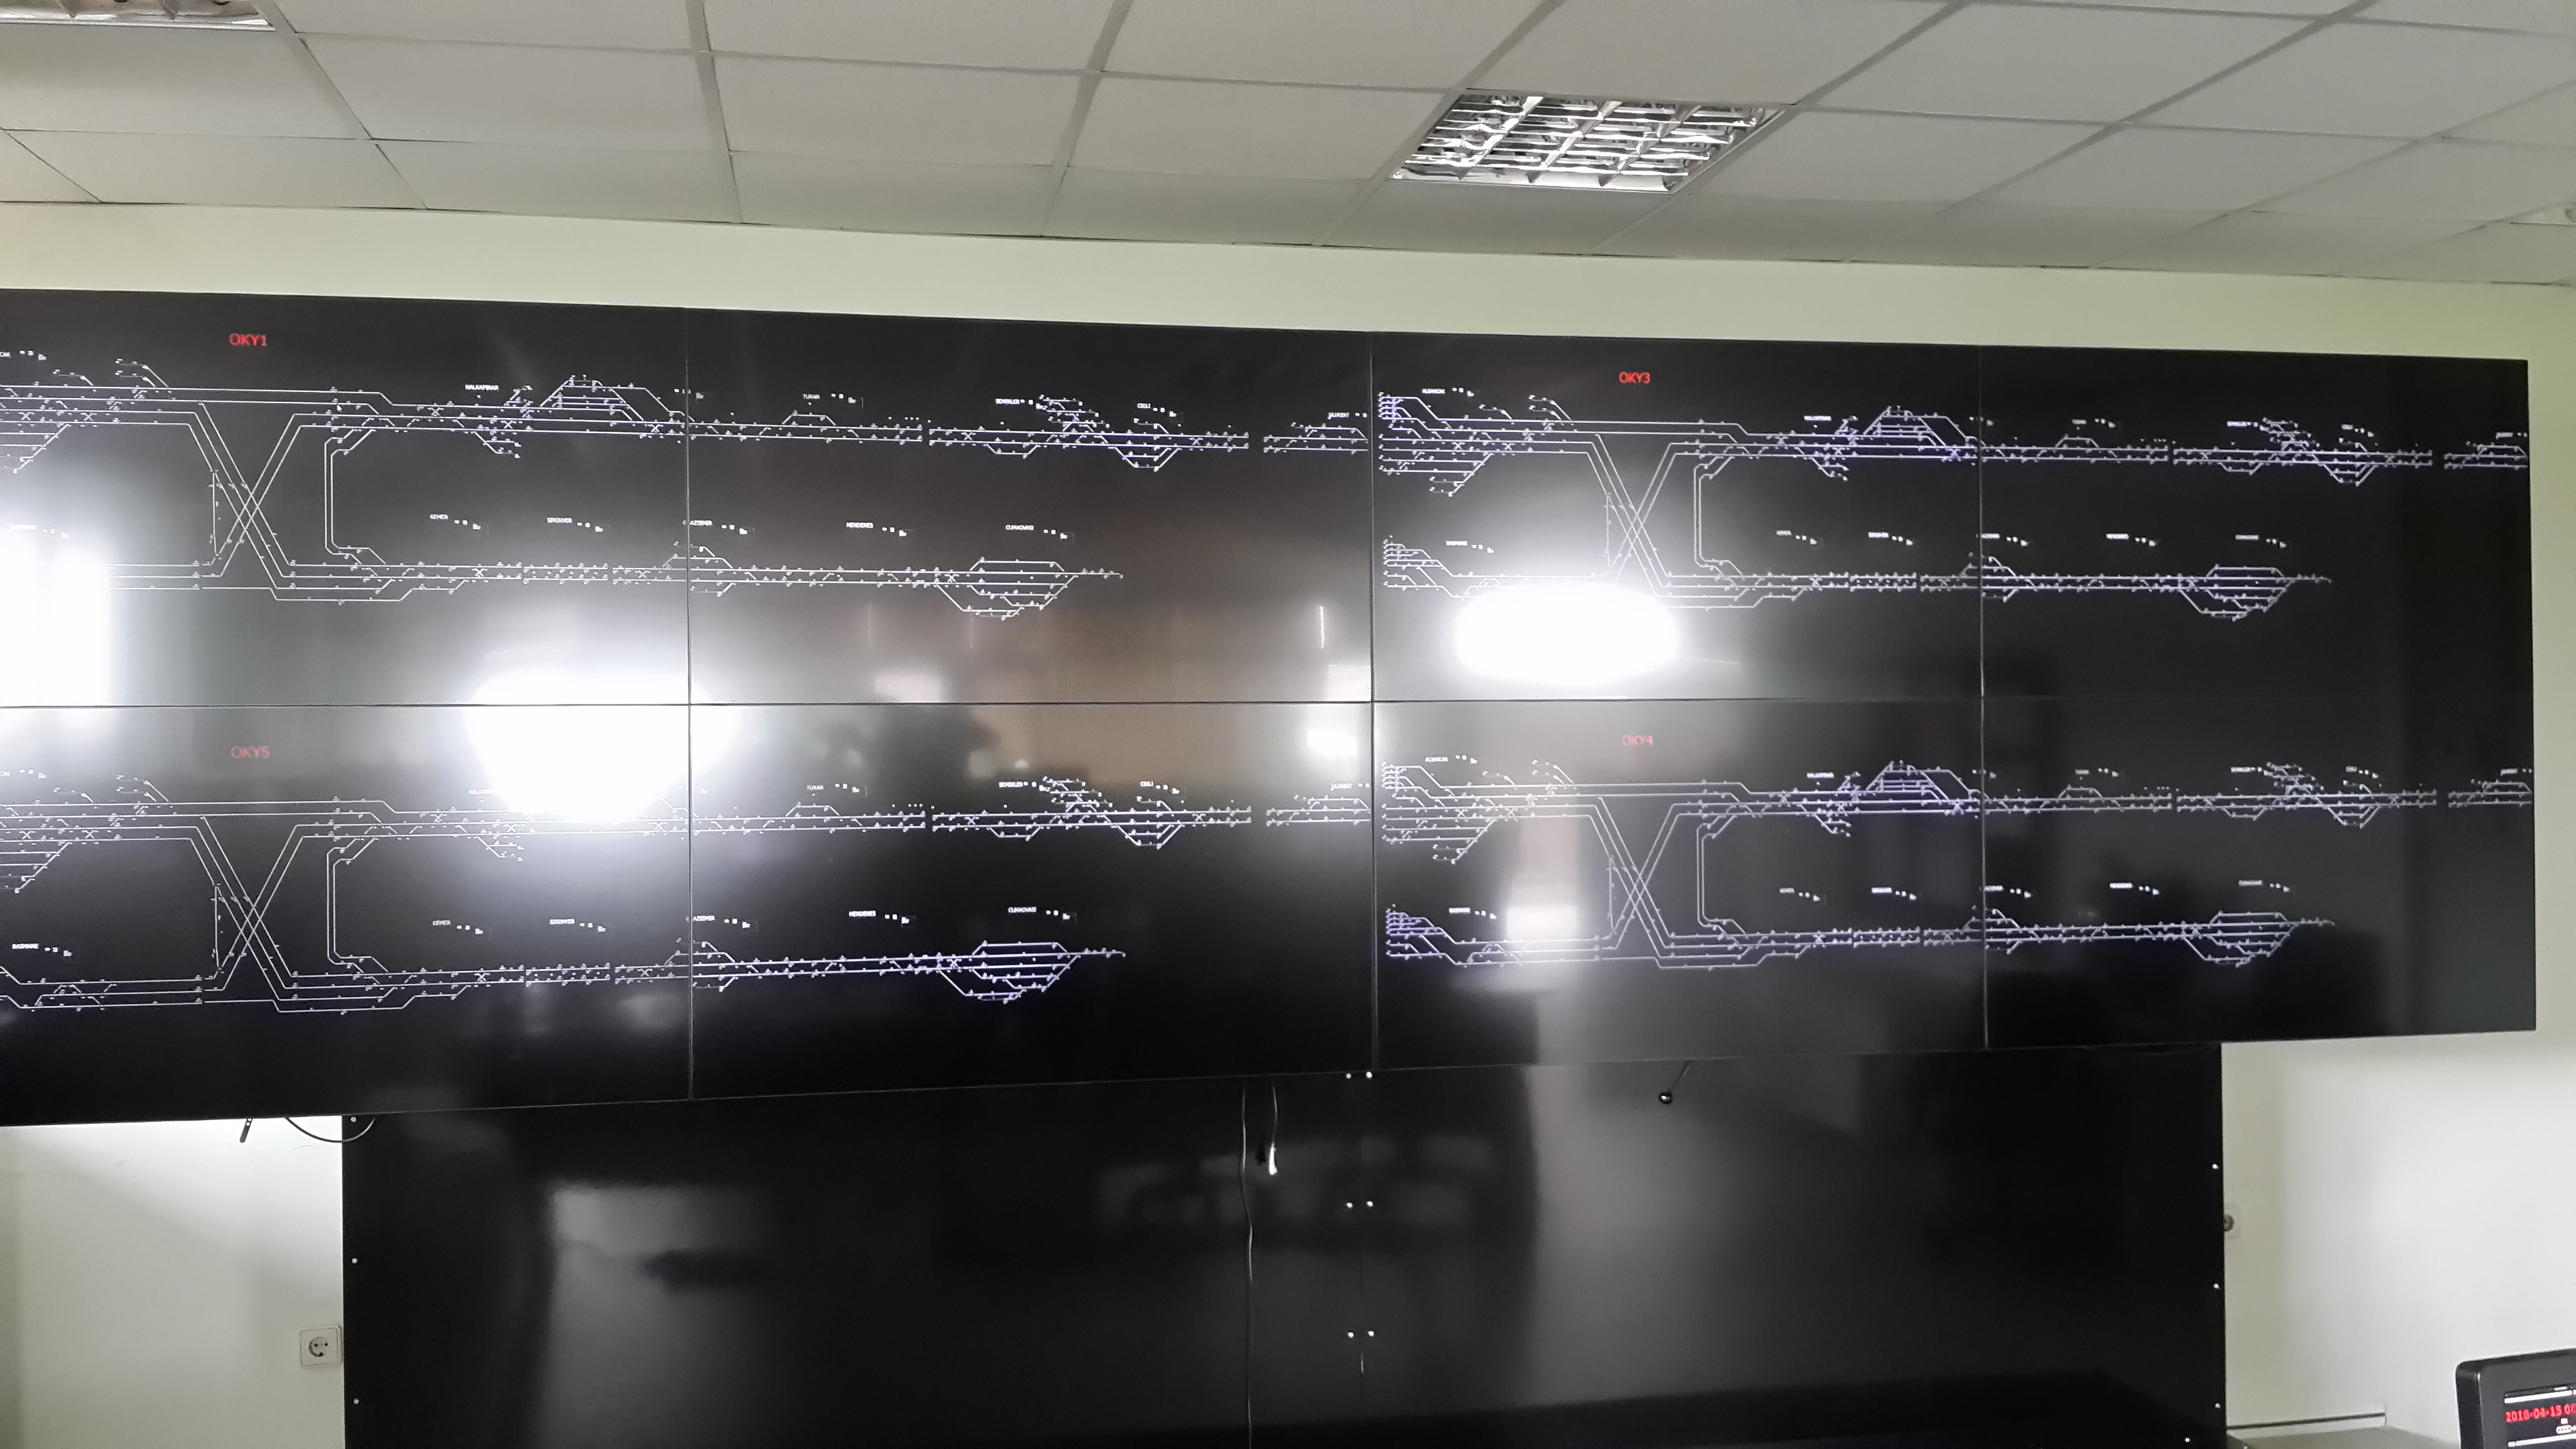
\includegraphics[width=8cm]{genisekranSonuc.jpg}
  \caption{4 farklı kullanıcıya ait ekran görüntülerinin geniş ekranda gösterimi}\label{fig:genisekranSonuc}
  
\end{figure}


\section{Conclusion}
Computer Simulations can be considered as a powerful tools for learning such as analysing, designing, and interacting. Especially in the vital criticality level it has become more important tools such as train traffic simulation.
The most important purpose of the train control system to prevent train collisions with other trains, keeping them in safe range.

The purpose of this study is to provide train traffic control in a distributed simulation system. The system consists of an instructor support five students and a scenario-editor. The system use real train route model located in Turkey.  During the simulation, dispatchers console can controls train traffic which have different  size and speed in system. Success in educational outcomes can be measured. Instructor console make decisions about the organization of teaching and learning experiences, classroom management, and responses to individual students. The user is able to monitor and track the progress of five targeted students throughout the course of the simulation.





% use section* for acknowledgment
\section*{Acknowledgment}


This work has been conducted within Rail Transit systems Simulation Research Lab- project (project number 3920-S513000) for Turkish State Railways, which is part of the Rail Transit Systems research program funded by The National Research Institute of Electronics and Cryptology (TUBITAK BILGEM). We thank all project partners for their work and contributions to the project.

\begin{thebibliography}{1}

\bibitem{FRISO}
A. D. Middelkoop and L. Loeve, “Simulation of traffic management with FRISO,” 2006, vol. 1, pp. 501–509.

\bibitem{ICVES}
M. Baohua, J. Wenzheng, C. Shaokuan, and L. Jianfeng, “A computer-aided multi-train simulator for rail traffic,” in IEEE International Conference on Vehicular Electronics and Safety, 2007. ICVES, 2007, pp. 1–5.
 
 
 

\end{thebibliography}




% that's all folks
\end{document}


